\chapter{Проектирование рентгенооптических трактов для Сибирского Кольцевого Источника Фонтов}

\section{Введение}
В данной главе мы рассмотрим схемы рентгенооптических трактов (здесь и далее, - бимлайнов), от источников высокого энергетических фотонов, - вставных устройств до деталей оптических компотен на билайне: фильтров, монохроматоров, рентгеновских зеркал. По большей части, будут обсуждаться станции первой очереди: 1-1 --- <<Микрофокус>>, 1-2 --- <<Структурная диагностика>>, 1-4 --- <<XAFS-спектроскопия и магнитный дихроизм>>.  

\section{Станция 1-4 --- <<XAFS-спектроскопия и магнитный дихроизм>>}
\subsection{Излучение клинообразного ондулятора}
В этой секции мы рассмотрим излучение из ондулятора специальной конструкции, который может дать широкий спектр. Идея в том, что разбить ондулятор на несколько секций с различным $K$ в каждой из них. Такая расстановка в первом приближении должна дать набор резонансов, которые должны сложиться в один сплошной спектр. Более детальное рассмотрение покажет, что в зависимости от корреляции фазы электрона между этими сегментами, могут проявляться интерференционные эффекты, которые в значительной степени будут изменять форму спектра. В нашем рассмотрении мы покажем влияние указанных вкладов для случая скачкообразного изменения поля, а также для классического случая клинообразного, т.н. зарубежной литературе tapered undulator.

Свои выкладки начнём с модифицированного интеграла~\ref{eq:field_dist_in_integral}, 
\begin{equation}
\begin{array}{lcl}
\vec{\widetilde{E}}_{\bot}(z_0,  \vec{r}_{\bot 0}, \omega) =
\cfrac{\omega eA_{JJ}}{2c^2z_0}\cfrac{K}{\gamma}
\displaystyle\int\limits_{-\lambda_w N/2}^{\lambda_w N/2} dz'
\exp[iCz'] 	\vec{e}_x,
\end{array}	
\end{equation} 
Здесь, для краткости выкладок, излучения мы сморим на оси, т.е. $\theta = 0$. В случае секционного ондулятора коэффициент ондуляторности меняется вдоль ондулятора, поэтому $K = K_0 + n\Delta K$, а также $C = C_0 + n\Delta C$, где $n$ --- это номер секции. $\Delta {C}$ введено следующим образом, помня $\omega_r = 2c\widetilde{\gamma}^2k_w$:
\begin{equation}
C =k_w\cfrac{\Delta \omega}{\omega_r} = \cfrac{\Delta \omega_r}{2c\gamma}\bigg(1 + \cfrac{(K_0 + n\Delta K)^2}{2}\bigg) \approx \cfrac{\Delta \omega_r}{2c\gamma}\bigg(1 + \cfrac{K^2_0}{2}(1 + \cfrac{n\Delta K}{K_0})\bigg) = C_0 + \Delta C
\end{equation} 
Секций, для условности, мы возьмём пять, и для удобства нумерацию будем вести $-2, -1, ... , 2$. Поэтому интеграл перепишеться в виде:
\begin{equation}
\begin{array}{lcl}
\vec{\widetilde{E}}_{\bot}(z_0,  \vec{r}_{\bot 0}, \omega) =
\cfrac{\omega eA_{JJ}}{2c^2 \gamma z_0}
\displaystyle\sum\limits_{n =-2}^{2}(K_0 + n\Delta K)
\displaystyle\int\limits_{(2n + 1)L_s/2}^{(2n - 1)L_s/2} dz'
\exp[i(C_0 + n\Delta C)z']	\vec{e}_x,
\end{array}	
\end{equation} 
Взяв интеграл, получим:
\begin{equation}
\begin{array}{lcl}
\vec{\widetilde{E}}_{\bot}(z_0,  \vec{r}_{\bot 0}, \omega) =
\cfrac{\omega eA_{JJ}}{2c^2 \gamma z_0}
\displaystyle\sum\limits_{n =-2}^{2}(K_0 + n\Delta K)
\sinc(\hat{C}/2)e^{in({C}_0 + n\Delta {C})L}	\vec{e}_x,
\end{array}	
\end{equation} 
Возведя в квадрат получим интенсивность:
\begin{equation}
\begin{array}{lcl}
{\widetilde{I}} =
\bigg(\cfrac{\omega eA_{JJ}}{2c^2 \gamma z_0}\bigg)^2\bigg[
\displaystyle\sum\limits_{n =-2}^{2}(K_0 + n\Delta K)^2\sinc^2(\hat{C_0} + n\Delta \hat{C}/2) + \\

\displaystyle\mathop{\sum\limits_{n, m =-2}^{2}}_{n \neq m}K^2_0\bigg(1 + n\cfrac{\Delta K}{K_0} + m\cfrac{\Delta K}{K_0}\bigg)
\sinc^2(\hat{C}/2)e^{i(n-m)\hat{C}_0 + (n^2 - m^2)\Delta \hat{C}}\bigg],
\end{array}	
\end{equation} 
Данное выражение можно проинтерпретировать следующим образом: первая сумма есть сумма сдвинутых по соответствующим резонансам $\sinc^2$ функций, вторая сумма отображает интерференцию между различными секциями ондулятора, и как кажется автору нежелательна. Данная комбинация приводит к хаотичным колебаниями в спектре, как показано на рис.~\ref{fig:section_und_analitics} пунктирными линиями, черной линей отмечана сумма $\sinc^2$ функций без учёта интерференционных слагаемых.
\begin{figure}
	\centering  
	\begin{minipage}{0.49\textwidth}
		\centering
		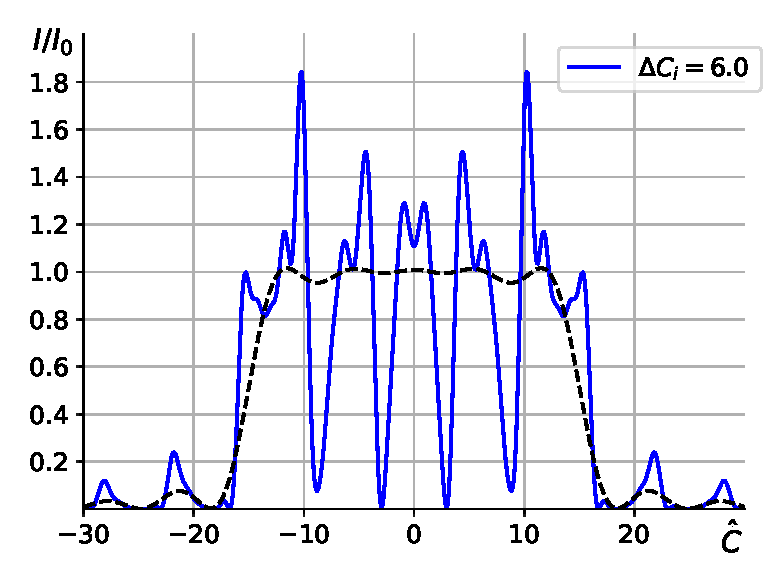
\includegraphics[width=\textwidth]{pic/spec_from_sec_und.pdf}
		\caption{}
		\label{fig:section_und_analitics}
	\end{minipage}\hfill
	\begin{minipage}{0.49\textwidth}
		\centering
		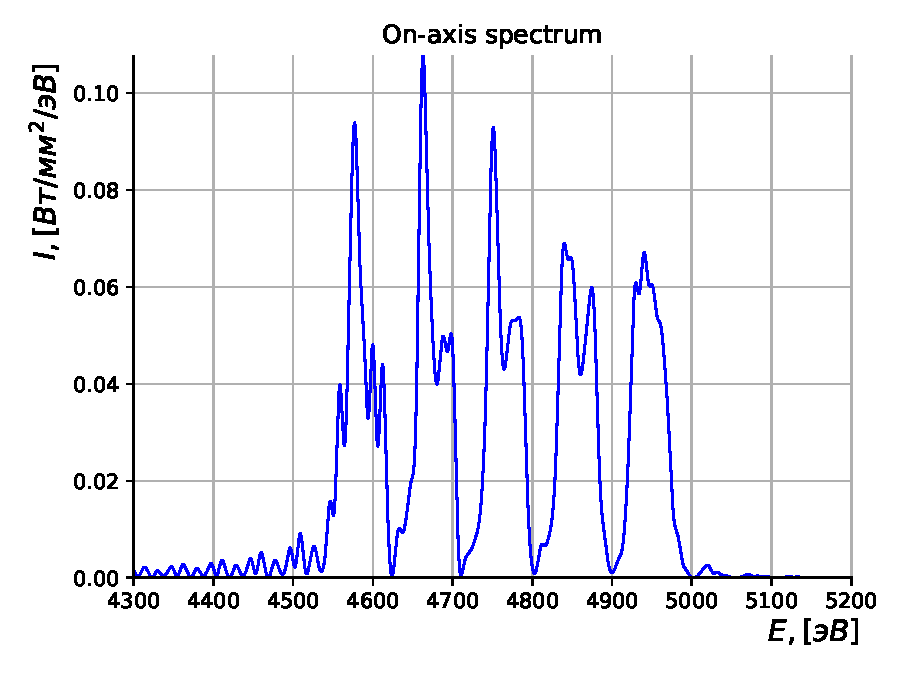
\includegraphics[width=\textwidth]{pic/sim_und_spec.pdf}
		\caption{}
		\label{fig:section_und_SRW}
	\end{minipage}    
\end{figure}
На рис.~\ref{fig:section_und_SRW} показан характерный спектр секционного ондулятора посчитанного при помощи симуляционного кода SRW. Сравнение формы синей пунктирной линии на рис.~\ref{fig:section_und_analitics} и кривой на рис.~\ref{fig:section_und_SRW} показывает, что были сделаны правильные предположения в нашей аналитической модели, происходит интерференция между различными частями ондулятора.
Один из возможных путей, чтобы избавиться от интерференционных слагаемых в спектре ондуляторного излучения, добавить произвольную фазу между секциями ондулятора. Дело в том, что данные вычисления проводились для ондного электрона, если если мы хотим получить спектр, который получиться в точке наблюдения, то можно понять, что спектры на рис.~\ref{fig:section_und_analitics} синими линиями необходимо усреднить по числу электронов в пучке, усреднение по большому числу электронов даст спектр, который будет являть простой суммой $\sinc^2$ до каких либо дополнительных фаз, результат усреднения, приведёт к чёрной линии на рис.~\ref{fig:section_und_analitics}. Теперь здесь надо визуально показать процесс усреднения и заключить, что именно такой спектр будет наблюдаться на источнике.
